\documentclass[ngerman]{scrartcl}
\usepackage{amsmath,amsthm,amssymb}
\usepackage[T1]{fontenc}
\usepackage[utf8]{inputenc}
\usepackage{lmodern}
\usepackage{graphicx}

\usepackage{hyperref}

\title{Berechenbare Analysis \\ Zusammenfassung \\ SoSe 19}
\author{Benedikt Lüken-Winkels}
\begin{document}

\maketitle
\tableofcontents

\newpage

%====================================
%
% SECTION
%
%====================================
\section{Berechenbarkeit}

%===========================
% SUBSECTION
%===========================
\subsection{Berechenbarkeit einer reellen Zahl}
Eine reelle Zahl ist dann berechenbar, wenn eine der \textbf{äquivalenten} Bedingungen erfüllt ist:
\begin{enumerate}
  \item \textbf{Binärdarstellung} Es gibt eine TM, die eine unendlich lange binäre Representation von $ x $ auf dem Ausgabeband erzeugt.
  \item \textbf{Fehlerabschätzung} Es gibt eine TM, die Approximationen liefert. Formal: $ q:\mathbb{N}\rightarrow \mathbb{Q} $ $ (q_{i})_{i \in \mathbb{N}} $ ist Folge rationaler Zahlen, die gegen $ x $ konvergiert. Bedeutet, dass alle $ q_i $ innerhalb eines bestimmten beliebig kleinen Bereichs um $ x $ liegen. Größter möglicher Fehler $ 2^0 = 1 $
  \item \textbf{Intervalschachtelung} Es gibt eine berechenbare Intervallschachtelung mit rationalen Endpunkten: Angabe zweier Folgen rationaler Zahlen mit der Bedingung, dass sie beide gegen $ x $ gehen und $ x $ dazwischen liegt. Ziel: Abstände von linker und rechter Schranke soll gegen null gehen.
  \item \textbf{Dedekindscher Schnitt} Menge $ \{q \in \mathbb{Q} | q < x \} $ ist entscheidbar. Beispiel $ \sqrt{2} $ ist berechenbar. $ \{ q | q < \sqrt{2} \} = \{ q | q^2 < 2\}$. $ \Rightarrow $ Es gibt einen Test, ob die Zahl kleiner ist.
  \item Man kann x als Summe von abzählbar unendlich vielen Brüchen darstellen: $ z \in \mathbb{Z} $ $ A \subseteq \mathbb{N} $, $ x_A = \sum_{i \in A} 2^{-i-1} $, $ x = z + x_A $
  \item Es exisitert eine \textbf{Kettenbruchentwicklung}
 \end{enumerate}
 \paragraph{Folgerungen / Beispiele}
\begin{itemize}
  \item $ \Rightarrow $ Für Berechenbarkeit muss nur eine der Bedingungen bewiesen werden. Menge der berechenbaren reelen Zahlen = $ \mathbb{R}_c $
  \item Nicht berechenbare reele Zahlen durch Diagonalisierung konstruierbar
  \item $ e $ berechenbar, weil die Fehlerabschätzung (2) existiert
  \item $ \pi $ (Notiert als alternierede Reihe) berechenbar, weil Intervalschachtelung existiert
  \item $ \sqrt{2} $ berechenbar, weil Dedekindscher Schnitt existiert.
 \end{itemize}

%===========================
% SUBSECTION
%===========================
\subsection{Mehrwertige Funktionen}
Mehrwertige Funktion $ f: \subseteq X \rightrightarrows  Y $ ist eine Funktion, die für ein x mehrere Werte für y haben kann. Ein Funktionswert eines x sind alle möglichen Werte aus Y.

\paragraph{Komposition von mehrwertigen Funktionen} In allen Fällen, muss das Ergebnis definiert sein. Definitionsbereich  der Komposition $ f \circ g $ sind die x und y, die in beiden Funktionen im Definitionsbereich liegen. Außerhalb des Definitionsbereichs dürfen die Funktionen 'machen was sie wollen'. Beispiele:
\begin{itemize}
  \item In der Implementierung: Approx von 2 und $ \sqrt{2} * \sqrt{2} $.
  \item Konversion von $ \mathbb{R} $ in Dezimalzahlen. Rundung mit erlaubter Schwankung ergibt verschiedene Ausgaben. Eindeutige Umwandlung (Rundung) ist nicht berechenbar, aber mehrwertig bb.
\end{itemize}

%===========================
% SUBSECTION
%===========================
\subsection{Berechenbare Folgen reeller Zahlen}
Modelle zur Realisierung: OTM, Typ-2-TM

\paragraph{Konvergenzmodul}
Wie schnell geht die Folge gegen einen Grenzwert $ \overline{x} = \lim_{i \rightarrow \infty} x_ i $.

Der Konvergenzmodul $ m : \mathbb{N} \rightarrow \mathbb{N} $ ergibt n für eine konvergente Folge $ (r_i)_{n \in \mathbb {N}}$, die gegen x konvergiert, für das gilt $ |x - r_i| < 2^{-n} $
\begin{itemize}
  \item bb Folge + bb Modul $ \Rightarrow $ Grenzwert bb
  \item bb Folge + \textbf{nicht} bb Modul $ \Rightarrow $ Grenzwert nicht bb. Lemma 4.30. Baue eine linksberechebare reelle Folge.
\end{itemize}

\subparagraph{Bestimmung des Konvergenzmoduls}

\paragraph{Konstruierte Folge $ (x_n)_n $} nicht-bb Grenzwert, aber monoton wachsend. Nicht berechenbarer Konvergenzmodul. \\
Die Funktion f ist auf den bb reellen Zahlen stetig, aber nicht bb mit einer nicht-bb kleinsten Nullstelle. Definitionsbereich von f ist $ \mathbb{R} ohne \{x_A \} $, also nicht stetig auf $ x_A $, da für $ x > x_A$ wird $ f(x) := 0$ gesetzt. Eigenschaften von f sind abhängig von A :
\begin{itemize}
  \item Ist A entscheidbar und der Definitionsraum ohne $ x_A $ ist berechenbar. (Sonst ist A ist so kompliziert, wie das Halteproblem und $ x_A $ kodiert das Halteproblem in einer reellen Zahl)
  \item A ist rekursiv-aufzählbar, aber nicht entscheidbar. f bildet die bb reellen Zahlen auf die bb reellen Zahlen ab.
\end{itemize}
Funktion bildet bb Zahlen auf bb Zahlen ab oder eine Funktion ist überall stetig, springt aber trotzdem. $ \Rightarrow $ Typ-2 bb-Modell wird bevorzugt um solche Probleme zu umgehen.

%===========================
% SUBSECTION
%===========================
\subsection{Berechenbare Mengen reeller Zahlen}
Für eine berechenbare Menge gibt es einen Algortihmus, der entscheidet, ob ein Element in einer Menge ist oder nicht, oder dann in eine Endlosschleife läuft (semi-entscheidbar). Typ-2-TM und OTM sind implementierbar. Nimmt man die Berechenbarkeit auf Typ-2-TM und OTM, gibt es keine Darstellung, für die Gleichheit \textbf{entscheidbar} ist. Auf diesem Berechenbarkeitsmodell sind die einzigen entscheidbaren Teilmengen von $ \mathbb{R}^k $, $ \mathbb{R}^k $ und $ \emptyset $, da die charakteristische Funktion $ \chi_A $ stetig sein muss und somit konstant 1 oder 0.

\paragraph{Entscheidbarkeit}
Eine Menge A aus X mit der Darstellung $ \delta_X $ heißt $ \delta_X $-entscheidbar, wenn die Funktion, die bestimmt, ob ein $ x \in A $, $(\delta_X, \rho)$-berechenbar ist. $(\rho, \rho) $-entscheidbare Teilmengen von $\mathbb{R}$ nennt man entscheidbar. $\Rightarrow $ Modifikation des Entscheidbarkeitsbegriffs, indem die charakteristische Funktion durch die Abstandsfunktion ersetzt wird.

\paragraph{Berechenbarkeit}
\begin{itemize}
  \item Eine abgeschlossene Menge heißt berechenbar, wenn sie leer ist oder der Abstand berechenbar ist.
  \item Eine offene Menge heißt berechenbar, wenn das Komplement der Menge berechenbar ist.
\end{itemize}


\paragraph{Plot von Mengen} Berechenbarkeit $ \Rightarrow $ Abstand berechenbar. Beispiel Mandelbrot/Julia-Menge. Wenn die Funktion geplottet werden kann man sie berechnen (effektive Stetigkeit)

\paragraph{Berechenbarer Graph $ \leftrightarrow $ Berechenbare Funktion}
Wenn $ f: \mathbb{R}^k \rightarrow \mathbb{R} $ eine totale Funktion ist, ist der Graph von f genau dann eine berechenbare abgeschlossene Menge, wenn f eine berechenbare Funktion ist.

%===========================
% SUBSECTION
%===========================
\subsection{Nichtberechenbare reelle Funktionen}
\paragraph{$ sign : \mathbb{R} \rightarrow \mathbb{R} $} sign ist nicht $ (\rho, \rho)$ berechenbar


%===========================
% SUBSECTION
%===========================
\subsection{Links/rechtsberechenbare reelle Zahlen}
Eine Reelle Zahl x ist linksberechebar, wenn $ \{q \in \mathbb{Q} | q < x  \}  $ rekursiv aufzählbar ist.  Eine Zahl ist berechenbar, genau dann wenn sie links und rechstberechenbar ist.


\paragraph{Vergleich mit berechenbaren reellen Zahlen}
Die Berechenbarkeiseigenschaft einer Zahl ergibt eine Intervallschachtelung (und umgekehrt)


%====================================
%
% SECTION
%
%====================================
\section{Effektive Stetigkeit}

\paragraph{Definition}
$ S \subseteq \mathbb{N} $ ist rekursiv aufzählbar.
\begin{enumerate}
  \item $ <i,j> \in S\ mit\ f(B^n(i))\subseteq B^1(j) $ erzeugt Rechtecke, durch die die Funktion laufen muss. Die Funktion liegt innerhalb der Schläuche.
  \item für jedes $ x\in Def(f) $ kann man ein $ <i,j> \in S $ finden. Die Schläuche werden beliebig fein.
\end{enumerate}

\paragraph{Definition}
\begin{itemize}
  \item Eine Funktion $ f: \subseteq \mathbb{R}^n \rightarrow \mathbb{R} $ ist genau dann berechenbar, wenn sie effektiv stetig ist.
  \item Aus Stetigkeit folgt Berechenbarkeit. Aus nicht Stetigkeit folgt nicht Berechenbarkeit
  \item Um nicht-Berechenbarkeit zu zeigem, zeigt man nicht-Stetigkeit
  \item Aus nicht-effektiver Stetigkeit folgt nicht-Berechenbarkeit. Bsp $  f(x) = 1, x \geq 0; 0, x < 0 $ ist nicht stetig und nicht berechenbar
\end{itemize}

\paragraph{Effektive Stetigkeit $ \Leftrightarrow $ Berechenbarkeit}
\begin{itemize}
  \item $ \Rightarrow $ Eine OTM M mit Eingabe n durchsucht S und das Orakel nach einem Tupel aus S und einem Wertpaar aus dem Orakel, sodass die Kugel aus dem Orakelwertpaar innerhalb der Kugel aus dem Tupel aus S, bei dem der Radius < $ 2^{-n}$ ist, liegt. Weil das Intervall aus <i,j> beliebig klein werden kann, ist liefert M so eine ausreichend genaue Approximation.
  \item $ \Leftarrow $ Eine OTM M sucht zu einer Eingabe <i,j>  und $ n\in \mathbb{N}$ eine Folge rationaler $ q_0,q_1,...,q_m$ Zahlen, sodass $ B^1(i) \subseteq B(q_k, 2^{-k}) $ wobei $ 0 \leq k \leq m $ und M ein $ \overline{q}_n $ liefert, bei dem $ B(\overline{q}_n, 2^{-n}) \subseteq B^1(j)$. m ist die Schranke für die Orakelanfragen. Die Folge umschließt B(i) und wird immer kleiner und enger um B(i).
  \begin{itemize}
    \item Bedingung 1: Nimm ein <i,j> aus S. Dann gibt es für $ x \in B^1(i) $ einen Namen $ \psi $ = $ \phi $ für $ k \leq m $. Bei dem $ f^\psi_M (n) $ ein $ \overline{p}_n $ liefert, sodass gilt: $ f(B^1(i)) \subset B(\overline{q}_n, 2^{-n}) \subseteq B^1(j) $.
    \item Bedingung 2: Wähle die Eingabe n so, dass gilt $ 2^{-n} < \epsilon $. Dann bildet der Schnitt aus allen Kuglen von $q_k$, B(i) und die Kugel um die Ausgabe von M $ \overline{q}_n $ ergibt B(j). Dadurch, dass für n gilt, dass $ 2^{-n} < \epsilon$, wird der Schlauch, den i und j aufspannen beliebig fein.
  \end{itemize}

\end{itemize}


%====================================
%
% SECTION
%
%====================================
\section{Berechenbare reelle Funktionen}
Wurzel: bei negativen Argumenten macht die OTM irgendetwas (undefiniert). Lösung: Die Approximation liefert eine rationale Zahl, die keine negativen Zahlen akzeptiert und


%====================================
%
% SECTION
%
%====================================
\section{Darstellung}

$ \delta(\phi) = x $ (OTM) $\delta(p) = x $ (Typ-2-TM), dann sind $ \phi, p\ \delta$-Namen von x


%===========================
% SUBSECTION
%===========================
\subsection{Cauchy-Darstellung}
$ M = [A \rightarrow B] $ ist die Menge aller partiellen Funktionen $ f : \subseteq A \rightarrow B $.

\paragraph{Definition} $ \rho : \subseteq[\mathbb{N}\rightarrow\mathbb{Q}] \rightarrow \mathbb{R}$

\begin{center}
  $ \rho(f) = x \Leftrightarrow (\forall i \in \mathbb{N})|x-f(i)|< 2^{-i}$ \\
  $ \rho $ = Cauchy-Darstellung der reellen Zahlen.
\end{center}

%====================================
%
% SECTION
%
%====================================
\section{Turingmaschinen (Berechenbarkeitsmodelle)}

%===========================
% SUBSECTION
%===========================
\subsection{Typ-2-Turingmaschinen}
Besonderheiten: Eingabeband ist read-only, Ausgabeband kann nur nach rechts schreiben. Undendliche Eingabe

\paragraph{Berechnete Funktion}
Eine Typ-2-TM M berechnet eine Funktion $ f_M: \subseteq \Sigma^w \rightarrow \Sigma^w $, die aus der Eingabe nach und nach die Ausgabe als Wort auf dem Ausgabeband erzeugt.

\begin{figure}[h]
  \centering
  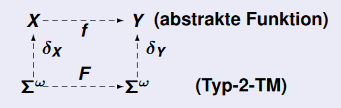
\includegraphics{typ2name.PNG}
  \caption{$ (\delta_X, \delta_Y)-berechenbar$ TYP-2-TM}
\end{figure}

%===========================
% SUBSECTION
%===========================
\subsection{Orakel-Turingmaschine OTM}
\paragraph{$ \mathbb{F} $}
ist die Menge aller partiellen Funktionen auf dem Alphabet der OTM: \\
 $ \mathbb{F} = \{ f | f: \subseteq \Sigma^* \rightarrow  \Sigma^* \}$
\paragraph{Funktion} Orakel als Eingabe und Parameter als Eingabe: Liefert Resultat

\paragraph{Berechnete Funktionen}
Eine OTM M berechnet eine Funktion $ f_M^\phi \in \mathbb{F}$, die bei der Eingabe w und einem Orakel $ \phi $ einen Endzustand v ohne Fehler erreicht. \\ $\Rightarrow$ für $ \phi \in Def(f\circ \delta_X) : f \circ \delta_X(\phi) = \delta_Y \circ \Gamma(\phi) $

\begin{figure}[h]
  \centering
  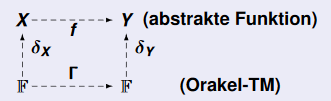
\includegraphics{orakelname.PNG}
  \caption{$ (\delta_X, \delta_Y)-berechenbar$ OTM}
\end{figure}


%===========================
% SUBSECTION
%===========================
\subsection{Komposition der Modelle}
$ \Gamma_3 = \Gamma_2 \circ \Gamma_1 $. $ \Gamma_3 $ muss $ \Gamma_2 $ das richtige Orakel liefern. Bei der Implementierung ruft $ \Gamma_3 $ das Approx von $ \Gamma_2 $ und $ \Gamma_2 $ wiederum das Approx von $ \Gamma_1 $ auf. \textbf{OTM und Implementierung sind das Gleiche.}

%====================================
%
% SECTION
%
%====================================

\section{Implementierung}
\textbf{Approx realisiert Orakelanfragen}

%===========================
% SUBSECTION
%===========================
\subsection{DAG Directed Acyclic Graph}
Acyclic, weil sonst um die Zahl zu berechnen, die Zahl selbst berechnet werden müsste.

\paragraph{Rundung} Naive multiplikatoin von rationalen Zahlen verdoppelt bei jeder Iteration den Speicherplatz $ \Rightarrow $ Rundung

\paragraph{Caching} Stuktur der DAGs ausnutzen. Bekannte Ergebnisse aus DAGs werden gespeichert (Anwendung bei der Komposition)

\paragraph{Limit-Operator} Modul ist konstant n wenn $ |f(n,x) - g(x)| < 2^{-n} $

\paragraph{Lambda-Funktionen} Funktionen als Eingabe für Variablen

%====================================
%
% SECTION
%
%====================================
\section{Allgemeines}

%===========================
% SUBSECTION
%===========================
\subsection{Abzählbar unendlich}
Es besteht eine Bijektion zu $ \mathbb{N} $.
\paragraph{Bemerkung} Es gibt so viele berechenbare reelle Zahlen, wie Programme

%===========================
% SUBSECTION
%===========================
\subsection{Entscheidbar}
Eine Menge M ist entscheidbar, wenn eine Funktion $ f_A : \mathbb{N} \rightarrow \mathbb{N} $ berechenbar ist und angibt, ob ein Element in der Menge ist, oder nicht. Bzw eine TM bei jeder Eingabe anhält.

%===========================
% SUBSECTION
%===========================
\subsection{Rekursiv aufzählbar}
Eine Menge M ist rekursiv aufzählbar, wenn eine Funktion $ f_A : \subseteq \mathbb{N} \rightarrow \mathbb{N} $ berechenbar ist und angibt, ob ein Element in der Menge ist, aber sonst undefiniert ist. Bzw eine TM bei einer korrekten Angabe anhält und sonst in eine Endlosschleife läuft.

%===========================
% SUBSECTION
%===========================
\subsection{$ \delta $-rekursiv-aufzählbar} Eine Orakel TM existiert, anhält wenn das Element aus der Menge ist.

%===========================
% SUBSECTION
%===========================
\subsection{Diagonalisierung}
\paragraph{$ \mathbb{R} $ ist überabzählbar}

Beweisidee: Man nimmt eine Folge reeller Zahlen zwischen 0 und 1. Mit der Diagonialisierung zeigt man, dass es eine Zahl gibt, die nicht in dieser Folge enthalten ist. Da dies für eine beliebige Menge geht, kann es keine Folge geben, die alle reellen Zahlen zwischen 0 und 1 enthält.

%===========================
% SUBSECTION
%===========================
\subsection{Isomorphismus}
Ein Isomorphismus ist zum Beispiel eine Funktion zwischen zwei Mengen, die bijektiv ist und ein Homomorphismus ist. Elemente der einen Menge werden auf bedeutungsgleiche Elemente der anderen Menge abgebildet.

%===========================
% SUBSECTION
%===========================
\subsection{Homomorphismus}
Ein Homomorphismus bildet die Elemente aus der einen Menge so in die andere Menge ab, dass sich ihre Bilder dort hinsichtlich der Struktur ebenso verhalten, wie sich deren Urbilder in der Ausgangsmenge verhalten.

%===========================
% SUBSECTION
%===========================
\subsection{Abgeschlossene Menge}
Eine Menge heißt abgeschlossen, wenn der Rand ein Teil der Menge ist. Die Menge ist berechenbar, wenn sie leer ist oder der Abstand $ (\rho, \rho_>) $-berechenbar ist.

%===========================
% SUBSECTION
%===========================
\subsection{Offene Menge}
Eine Menge heißt offen, wenn kein Element der menge auf ihrem Rand liegt. Die Menge ist berechenbar, wenn das Komplement berechenbar ist.

%===========================
% SUBSECTION
%===========================
\subsection{Kompakte Menge}

%===========================
% SUBSECTION
%===========================
\subsection{Chomsky-Hierarchie}
\begin{itemize}
  \item Typ-0: Beliebige formale Grammatik. Rekursiv aufzählbar
  \item Typ-1: Kontextsensitive Grammatik
  \item Typ-2: Kontextfreie Grammatik
  \item Typ-3: Reguläre Grammatik
\end{itemize}




%====================================
%
%
%        END DOCUMENT
%
%
%====================================
\end{document}
